\documentclass{standalone}
\usepackage{tikz}
\usetikzlibrary{fit}
\usetikzlibrary{shapes.geometric}

\usepackage[dvipsnames]{xcolor}
\newcommand\x{9}
\newcommand\y{3}
\begin{document}
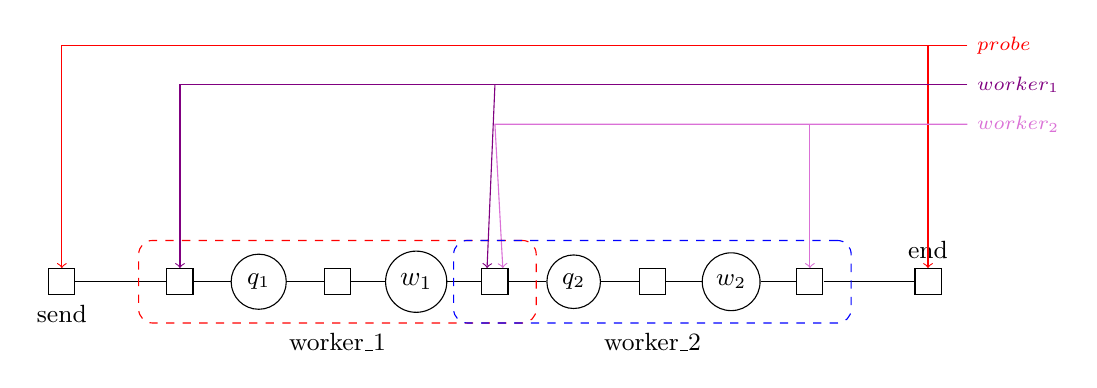
\begin{tikzpicture}[square/.style={regular polygon,regular polygon sides=4}, box/.style = {draw,red, dashed, inner sep=10pt,rounded corners=5pt}]

    \node[label=below:{\small send}] at (-2.5, 0) [square, draw] (s_1) {};
    \node at (-1, 0) [square, draw] (sw) {};
    \node at (0, 0) [circle, minimum size = 0.7cm, draw] (q_1) {\small $q_1$}; 
    \node at (1, 0) [square, draw] (e_1) {};
    \node at (2, 0) [circle, draw] (w_1) {$w_1$};
    \node at (3, 0) [square, draw] (e_2) {};

    \node at (4, 0) [circle, draw] (q_2) {\small $q_2$};
    \node at (5, 0) [square, draw] (e_3) {};
    
    \node at (6, 0) [circle, draw] (w_2) {\small $w_2$};
    \node[label={\small end}] at (8.5, 0) [square, draw] (e_4) {};
    \node at (7, 0) [square, draw] (ew2) {};
    
    
    %Probe 1
    \draw[->, red] (\x, \y) node[right] {\scriptsize $probe$} -- (-2.5, \y) -- (s_1.north) ;
    \draw[->, red] (8.5, \y) -- (e_4.north);

    %Probe 2
    \draw[->, violet] (\x, \y - 0.5) node[right] {\scriptsize$worker_1$} -- (-1, \y - 0.5) -- (sw.north);
    \draw[->, violet] (3, \y - 0.5) -- ([xshift=-0.1cm]e_2.north);

    % Probe 3
     \draw[->, Orchid] (\x, \y - 1) node[right] {\scriptsize $worker_2$} -- (3, \y - 1) -- ([xshift=0.1cm]e_2.north);
    \draw[->, Orchid] (7, \y - 1) -- (ew2.north);


    \draw (s_1.east) -- (sw.west);
    \draw (sw.east) -- (q_1.west);
    \draw (q_1.east) -- (e_1.west);
    \draw (e_1.east) -- (w_1.west);
    \draw (w_1.east) -- (e_2.west);
    \draw (e_2.east) -- (q_2.west);
    \draw (q_2.east) -- (e_3.west);
    \draw (e_3.east) -- (w_2.west);
    \draw (w_2.east) -- (ew2.west);
    \draw (ew2.east) -- (e_4.west);
    
    \node[label=below:{\small worker\_1}, box, fit=(sw)(e_2)] {};
    \node[label=below:{\small worker\_2}, box, blue, fit=(e_2)(ew2)] {};
\end{tikzpicture}

\end{document}

